\documentclass[brazilian,11pt]{article}

\usepackage{babel}
\usepackage[utf8]{inputenc}
\usepackage[T1]{fontenc}
\usepackage{lmodern}

\usepackage{graphicx}
\setkeys{Gin}{keepaspectratio}

\usepackage{amssymb,amsfonts,amsmath}
\usepackage{mathtools}

\usepackage{tikz}
\usetikzlibrary{calc}

\usepackage{siunitx}
\sisetup{locale = FR}

\newcommand{\esima}{\textordfeminine }
\newcommand{\esimo}{\textordmasculine }

\newcommand{\vboxcorr}[2]{%
    \resizebox{!}{\totalheight-#1}{#2}%
}
\newcommand{\hboxcorr}[2]{%
    \resizebox{\width-#1}{!}{#2}%
}

\begin{document}

\section*{Resolução da 3.12}
\begin{itemize}
    \item Precisamos encontrar a área da região avermelhada \(A\) como uma 
        função de \(h\)
        \begin{center}
            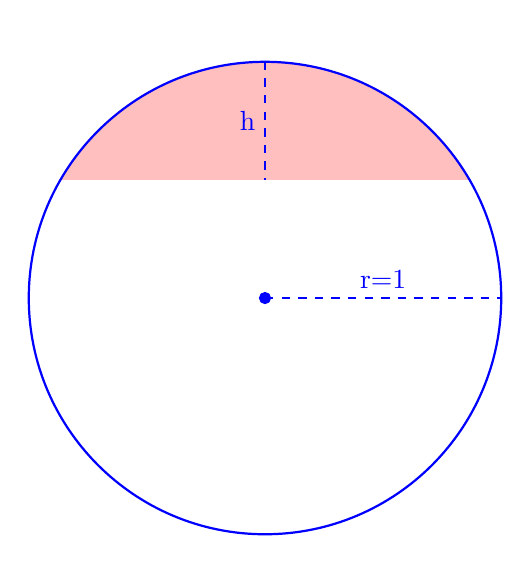
\begin{tikzpicture}
                \filldraw [red!25] (0,0) ++(150:3cm) arc (150:30:3cm);
                \filldraw [blue] (0,0) circle (2pt);
                \draw [blue, dashed] (0,0) -- node [above, midway] {r=1} (3cm,0);
                \draw [blue, dashed] (0,3cm) -- node[left,midway] {h} (0,1.5cm) ;
                \draw [blue, thick] (0,0) circle (3cm);
            \end{tikzpicture}
        \end{center}
    \item Seja \(B\) a área da região esverdeada
        \begin{center}
            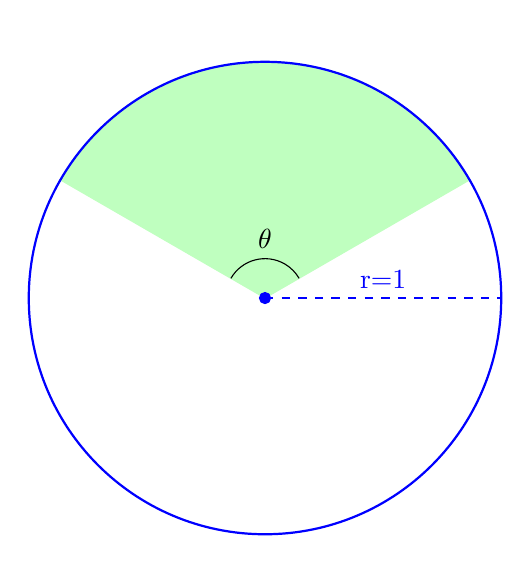
\begin{tikzpicture}
                \filldraw [green!25] (0,0) -- (150:3cm) arc (150:30:3cm) -- cycle;
                \draw (0,0) ++(150:0.5cm) arc (150:30:0.5cm) node [midway, above] {$\theta$};
                \filldraw [blue] (0,0) circle (2pt);
                \draw [blue, dashed] (0,0) -- node [above, midway] {r=1} (3cm,0);
                \draw [blue, thick] (0,0) circle (3cm);
            \end{tikzpicture}
        \end{center}
    \item Usando regra de três e o fato que quando \(\theta = 2\pi\) 
        a área é igual a \(\pi r^2\)

        \[
            \begin{matrix}
                2\pi ~\rule{1cm}{1pt}~ \pi r^2 \\
                \theta ~\rule{1cm}{1pt}~ B
            \end{matrix}
            \implies B = \frac{\theta}{2}r^2
        \]

    \item Seja \(C\) a área da região azulada
        \begin{center}
            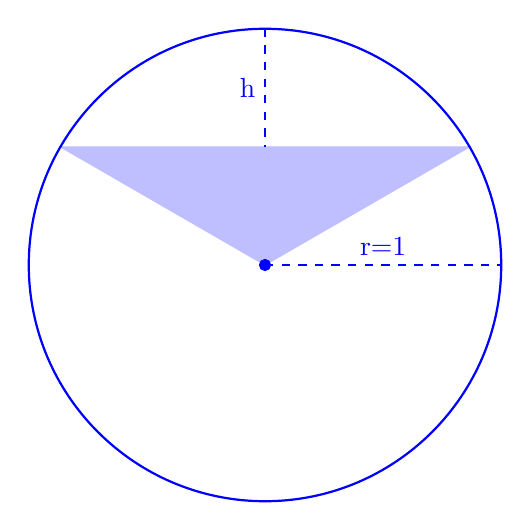
\begin{tikzpicture}
                \filldraw [blue!25] (0,0) -- (150:3cm) -- (30:3cm) -- cycle;
                \draw [blue, dashed] (0,3cm) -- node[left,midway] {h} (0,1.5cm) ;

                \filldraw [blue] (0,0) circle (2pt);
                \draw [blue, dashed] (0,0) -- node [above, midway] {r=1} (3cm,0);
                \draw [blue, thick] (0,0) circle (3cm);
            \end{tikzpicture}
        \end{center}

    \item Da figura, temos que a altura do triângulo é \(r-h\) e o comprimento
        da base \(b\) pode ser calculada usando o teorema de Pitágoras com
        hipotenusa \(r\), um cateto igual a \(r-h\) e o outro cateto igual a
        metade do comprimento da base \(b/2\). Ou seja
        \[
            r^2 = (r-h)^2 + \left(\frac{b}{2}\right)^2 \implies
            b=2\sqrt{r^2-(r-h)^2}
        \]
    \item A área do triângulo é dada base vezes altura dividido por 2, de forma que
        \[
            C=\frac{(r-h)\times 2\sqrt{r^2-(r-h)^2}}{2} \implies
            C=(r-h) \sqrt{r^2-(r-h)^2}
        \]
    \item Das figuras

        \hboxcorr{52pt}{
            \begin{minipage}{0.3\textwidth}
                \hboxcorr{80pt}{
                    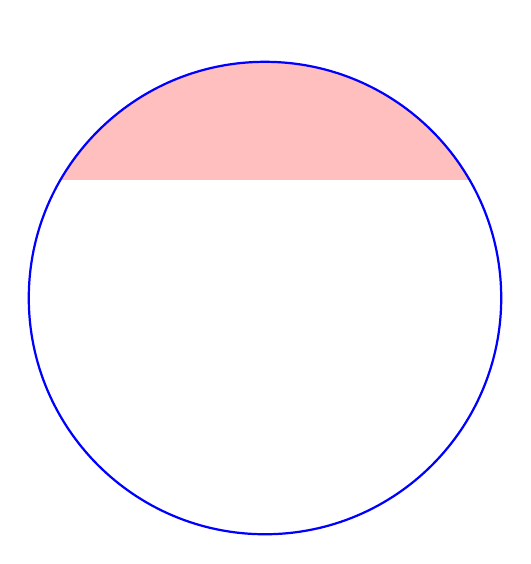
\begin{tikzpicture}
                        \filldraw [red!25] (0,0) ++(150:3cm) arc (150:30:3cm);
                        \draw [blue, thick] (0,0) circle (3cm);
                    \end{tikzpicture}
                }
            \end{minipage}%
            \huge{=}
            \begin{minipage}{0.3\textwidth}
                \hboxcorr{80pt}{
                    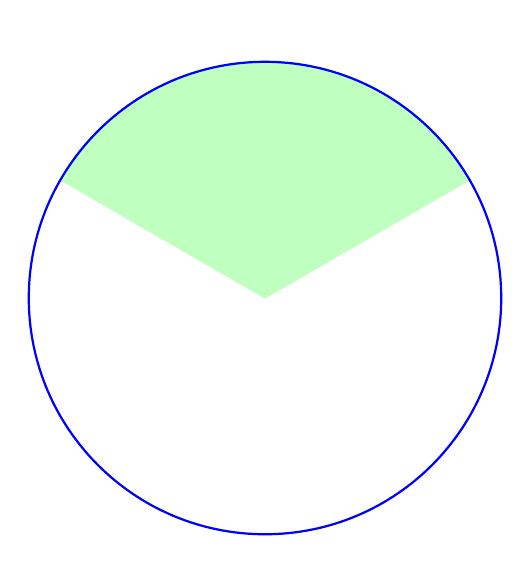
\begin{tikzpicture}
                        \filldraw [green!25] (0,0) -- (150:3cm) arc (150:30:3cm) -- cycle;
                        \draw [blue, thick] (0,0) circle (3cm);
                    \end{tikzpicture}
                }
            \end{minipage}
            \huge{\textbf{--}}
            \begin{minipage}{0.3\textwidth}
                \hboxcorr{80pt}{
                    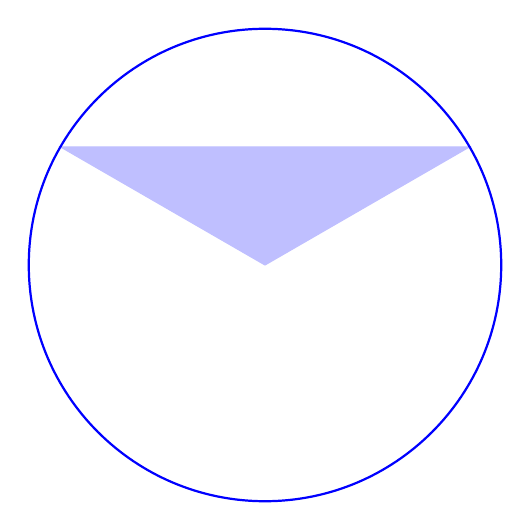
\begin{tikzpicture}
                        \filldraw [blue!25] (0,0) -- (150:3cm) -- (30:3cm) -- cycle;

                        \draw [blue, thick] (0,0) circle (3cm);
                    \end{tikzpicture}
                }
            \end{minipage}
        }
    \item Ou seja \(A=B-C\)
        \[
            A=
            \frac{\theta}{2}r^2
            -
            (r-h) \sqrt{r^2-(r-h)^2}
        \]
    \item Para encontrar \(\theta\) como função de \(h\) observamos que 
        no triângulo
        \begin{center}
            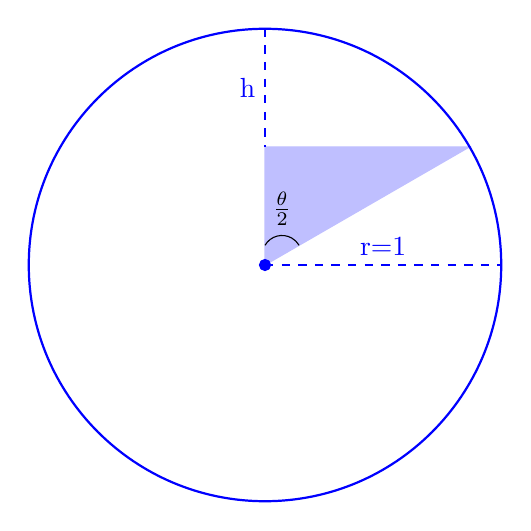
\begin{tikzpicture}
                \path (0,0) -- (150:3cm) coordinate (A) -- (30:3cm) coordinate (B) -- cycle;
                \filldraw [blue!25] (0,0) -- ($(A)!0.5!(B)$) -- (30:3cm) -- cycle;
                \draw [blue, dashed] (0,3cm) -- node[left,midway] {h} (0,1.5cm) ;
                \draw (0,0) ++(90:0.25cm) arc (150:30:0.25cm) node [midway, above] {$\frac{\theta}{2}$};

                \filldraw [blue] (0,0) circle (2pt);
                \draw [blue, dashed] (0,0) -- node [above, midway] {r=1} (3cm,0);
                \draw [blue, thick] (0,0) circle (3cm);
            \end{tikzpicture}
        \end{center}
        temos que
        \[
            \cos{\frac{\theta}{2}}=\frac{r-h}{r} \implies
            \frac{\theta}{2}=\arccos{\left(\frac{r-h}{r}\right)}
        \]
    \item Finalmente, temos que
        \footnote{Uma outra forma de abordar esse problema seria considerar uma 
        circunferência centrada na origem \(x^2+y^2=r^2\) e calcular
        \[
            \int_{r-h}^{r} \sqrt{r^2-x^2}\; dx
        \]
        que é a metade da área procurada \(A\). Essa abordagem fica como 
        exercício de Cálculo para os interessados.
        }
        \[
            A=
            r^2\arccos{\left(\frac{r-h}{r}\right)}
            -
            (r-h) \sqrt{r^2-(r-h)^2}
        \]
    \item Lembrando que 
        \[
            dA=\frac{dA}{dh} dh
        \]
        e que 
        \begin{align*}
            \frac{d}{dx}\arccos x &= -\frac{1}{\sqrt{1-x^2}} \\
            \frac{d}{dx}\sqrt{x} &=\frac{1}{2\sqrt{x}}
        \end{align*}
        temos que
        \[
            \begin{split}
                \frac{dA}{dh} =&
                \frac{d}{dh}\left[
                    r^2\arccos{\left(\frac{r-h}{r}\right)}
                    -
                    (r-h) \sqrt{r^2-(r-h)^2}
                    \right] \\
                =&r^2\frac{d}{dh}\arccos{\left(\frac{r-h}{r}\right)}
                -
                \frac{d}{dh}\left[
                    (r-h) \sqrt{r^2-(r-h)^2}
                \right] \\
            =&-r^2\frac{1}{\sqrt{1-\left(\frac{r-h}{r}\right)^2}}
                \left(-\frac{1}{r}\right)-\\
                &r\frac{1}{2\sqrt{r^2-(r-h)^2}}
                [-2(r-h)(-1)]+\\
                &\sqrt{r^2-(r-h)^2}+
                h\frac{1}{2\sqrt{r^2-(r-h)^2}}
                [-2(r-h)(-1)]\\
                =&\frac{r^2}{\sqrt{r^2-(r-h)^2}}-
                \frac{(r-h)(r-h)}{\sqrt{r^2-(r-h)^2}}+
                \sqrt{r^2-(r-h)^2} \\
                =&2\sqrt{r^2-(r-h)^2} \\
                =&2\sqrt{2rh-h^2}
            \end{split}
        \]
    \item Ou seja, \(dA=2\sqrt{2rh-h^2}dh\)
    \item Para simplificar as contas usaremos o 
        fato de que \(r=1\) \textit{para este problema}
    \item Temos que
        \begin{align*}
            dF&=PdA = \rho g h dA = 2\rho g h \sqrt{2h-h^2} dh \\
            d\tau&=h dF = \rho g h^2 dA= 2\rho g h^2 \sqrt{2h-h^2} dh \\
        \end{align*}
        onde \(0 \leq h \leq 2r\)

    \item Primeiro, temos que
        \[
            \int_0^{2r} h\sqrt{2h-h^2}\; dh
        \]
        pode ser associada ao triângulo 
        \begin{center}
            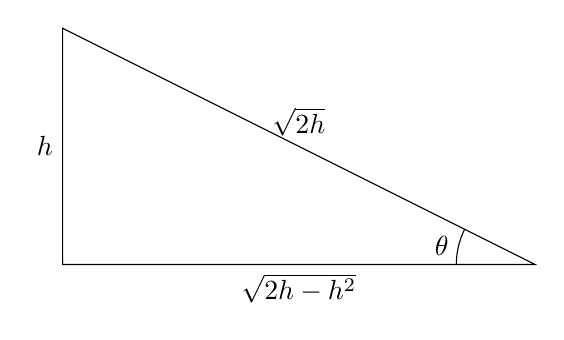
\begin{tikzpicture}
                \draw (0,0) -- node [midway, left] {$h$} (0,3cm) 
                -- node [midway, above] {$\sqrt{2h}$} (6cm,0) 
                -- node [midway, below] {$\sqrt{2h-h^2}$} cycle;
                \draw (6cm,0) ++ (180:1cm) arc (180:180+atan2(-1,2):1cm) 
                node [midway, left] {$\theta$};
            \end{tikzpicture}
        \end{center}
        de forma que
        \begin{align*}
            \sin \theta &= \frac{h}{\sqrt{2h}}=\frac{\sqrt{h}}{\sqrt{2}}
            \implies \cos{\theta}d\theta = \frac{dh}{\sqrt{8}\sqrt{h}} 
            \implies dh=4\sin\theta\cos\theta d\theta\\
            \cos\theta &= \frac{\sqrt{2h-h^2}}{\sqrt{2h}}
            \implies 2\sin\theta\cos\theta=\sqrt{2h-h^2}
        \end{align*}
    \item Ou seja \(\sqrt{2h-h^2}dh=8\sin^2\theta\cos^2\theta d\theta\)
        e \(h=2\sin^2\theta\)
    \item Além disso, temos que
        \begin{align*}
            & h=0 \implies \theta=0 \\
            & h=2 \implies \sin\theta = 1 \implies \theta = \frac{\pi}{2}
        \end{align*}
        de forma que
        \[
            \begin{split}
                \int_0^{2} h\sqrt{2h-h^2}\; dh &=
                16\int_0^{\pi/2}\sin^4\theta\cos^2\theta\;d\theta \\
                &= 16\int_0^{\pi/2}(\sin^4\theta-\sin^6\theta)\; d\theta
            \end{split}
        \]
    \item Na integral \(\int \sin^n x\; dx\) podemos considerar
        \(u=\sin^{n-1}x\) e \(dv=\sin x\; dx\) o que nos dá
        \(du=(n-1) \sin^{n-2}\cos x\; dx\) e 
        \(v=-\cos x\). Ou seja, 
        \(v\;du=-(n-1)\sin^{n-2}\cos^2\;dx=(1-n)(\sin^{n-2} x - \sin^n x)\; dx\)
    \item Integrando por partes \(\int \sin^n\;  dx\), temos
        \[
            n\int \sin^n x\; dx = -\sin^{n-1} x \cos x-
            (1-n)\int\sin^{n-2} x\; dx
        \]
        ou seja
        \[
            \int \sin^n x\; dx = -\frac{1}{n} \sin^{n-1} x\cos x+
            \frac{n-1}{n}\int\sin^{n-2} x\; dx
        \]
    \item Assim
        \begin{align*}
            \int \sin^6\theta\; d\theta&=
            -\frac{1}{6}\sin^5 \theta\cos\theta+
            \frac{5}{6}\int\sin^4 \theta\; d\theta \\
            \int\sin^6\theta\; d\theta-\int\sin^4\theta\;d\theta&=
            -\frac{1}{6}\sin^5 \theta\cos\theta-
            \frac{1}{6}\int\sin^4 \theta\; d\theta \\
            \int\sin^4\theta\; d\theta&=-\frac{1}{4}\sin^3\theta\cos\theta+
            \frac{3}{4}\int\sin^2\theta\;d\theta \\
            \int\sin^2\theta\;d\theta &=-\frac{1}{2}\sin\theta\cos\theta+
            \frac{1}{2}\int d\theta \\
            \int\theta\; d\theta &= \theta
        \end{align*}
    \item Ou seja
        \[
            16\int_0^{\pi/2}(\sin^4\theta-\sin^6\theta)\; d\theta =
            0+0+0+16\times\frac{\pi}{2}\times\frac{1}{2}\times\frac{3}{4}\times\frac{1}{6}=
            \frac{\pi}{2}
        \]
        e portanto
        \[
            \int_0^2 2h\sqrt{2h-h^2}\; dh = \pi
        \]
    \item Finalmente, temos que
        \[
            F=\rho g 
            \int_0^2 2h\sqrt{2h-h^2}\; dh = 
            9.8 \times 1000 \times \pi = \SI{30787.6}{N}
        \]
    \item Aproveitando os passos utilizados na integral anterior, temos que
        \[
            \begin{split}
                \int_0^{2} h^2\sqrt{2h-h^2}\; dh &=
                32\int_0^{\pi/2}\sin^6\theta\cos^2\theta\;d\theta \\
                &= 32\int_0^{\pi/2}(\sin^6\theta-\sin^8\theta)\; d\theta
            \end{split}
        \]
        e que
        \begin{align*}
            \int \sin^8\theta\; d\theta&=
            -\frac{1}{8}\sin^7 \theta\cos\theta+
            \frac{7}{8}\int\sin^6 \theta\; d\theta \\
            \int\sin^8\theta\; d\theta-\int\sin^6\theta\;d\theta&=
            -\frac{1}{8}\sin^7 \theta\cos\theta-
            \frac{1}{8}\int\sin^6 \theta\; d\theta \\
            \int \sin^6\theta\; d\theta&=
            -\frac{1}{6}\sin^5 \theta\cos\theta+
            \frac{5}{6}\int\sin^4 \theta\; d\theta \\
            \int\sin^4\theta\; d\theta&=-\frac{1}{4}\sin^3\theta\cos\theta+
            \frac{3}{4}\int\sin^2\theta\;d\theta \\
            \int\sin^2\theta\;d\theta &=-\frac{1}{2}\sin\theta\cos\theta+
            \frac{1}{2}\int d\theta \\
            \int\theta\; d\theta &= \theta
        \end{align*}

    \item Ou seja
        \[
            32\int_0^{\pi/2}(\sin^6\theta-\sin^8\theta)\; d\theta =
            0+0+0+0+
            32\times\frac{\pi}{2}\times\frac{1}{2}\times\frac{3}{4}
            \times\frac{5}{6}\times\frac{1}{8} = \frac{5\pi}{8}
        \]
        e portanto
        \[
            \int_0^2 2h^2\sqrt{2h-h^2}\; dh = \frac{5\pi}{4}
        \]
    \item Assim, temos que
        \[
            \tau=\rho g 
            \int_0^2 2h^2\sqrt{2h-h^2}\; dh = 
            9.8 \times 1000 \times \frac{5\pi}{4}
        \]
        e que
        \[
            F h_{cp} = \tau \implies 
            9.8 \times 1000 \times \pi \times h_{cp} =
            9.8 \times 1000 \times \frac{5\pi}{4}
        \]
        de forma que
        \[
            h_{cp}=\frac{5}{4}
        \]
\end{itemize}

\end{document}
